% !TEX root = ../../main.tex


\begin{figure}[p]
\vspace*{-5pt}
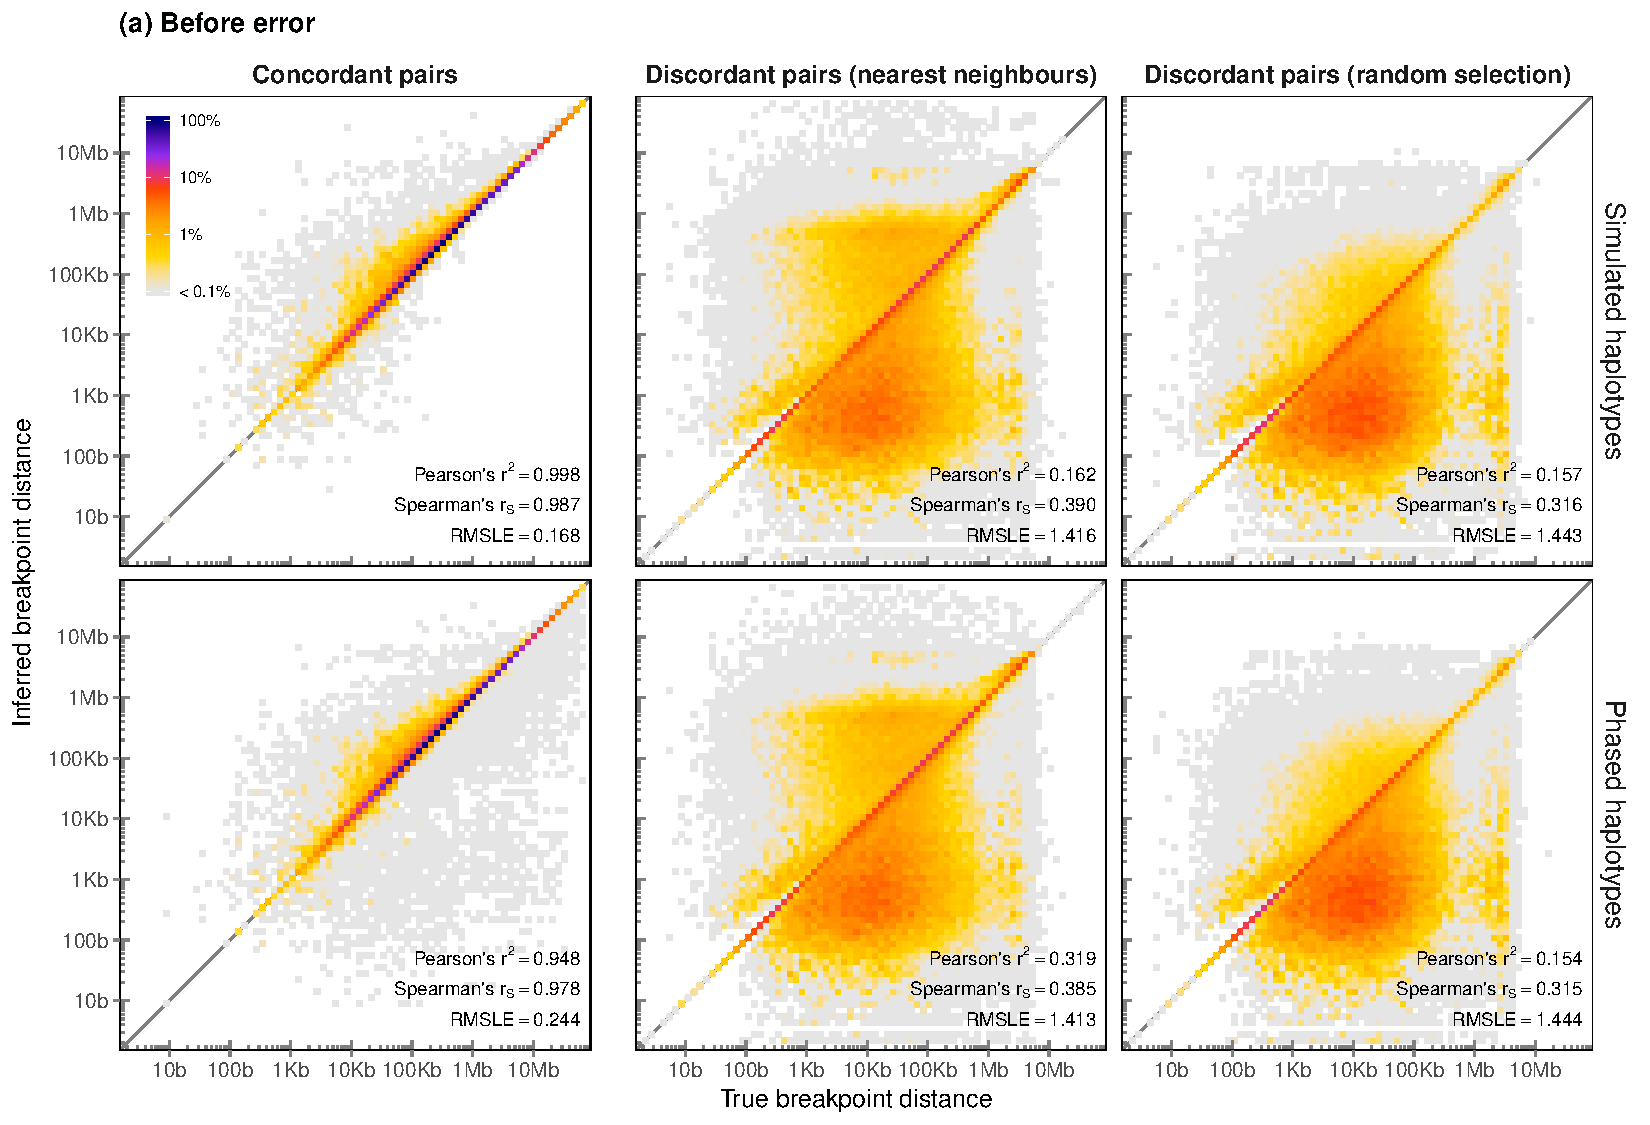
\includegraphics[width=\textwidth]{./img/ch5/hhmm_ibd_rel_A}
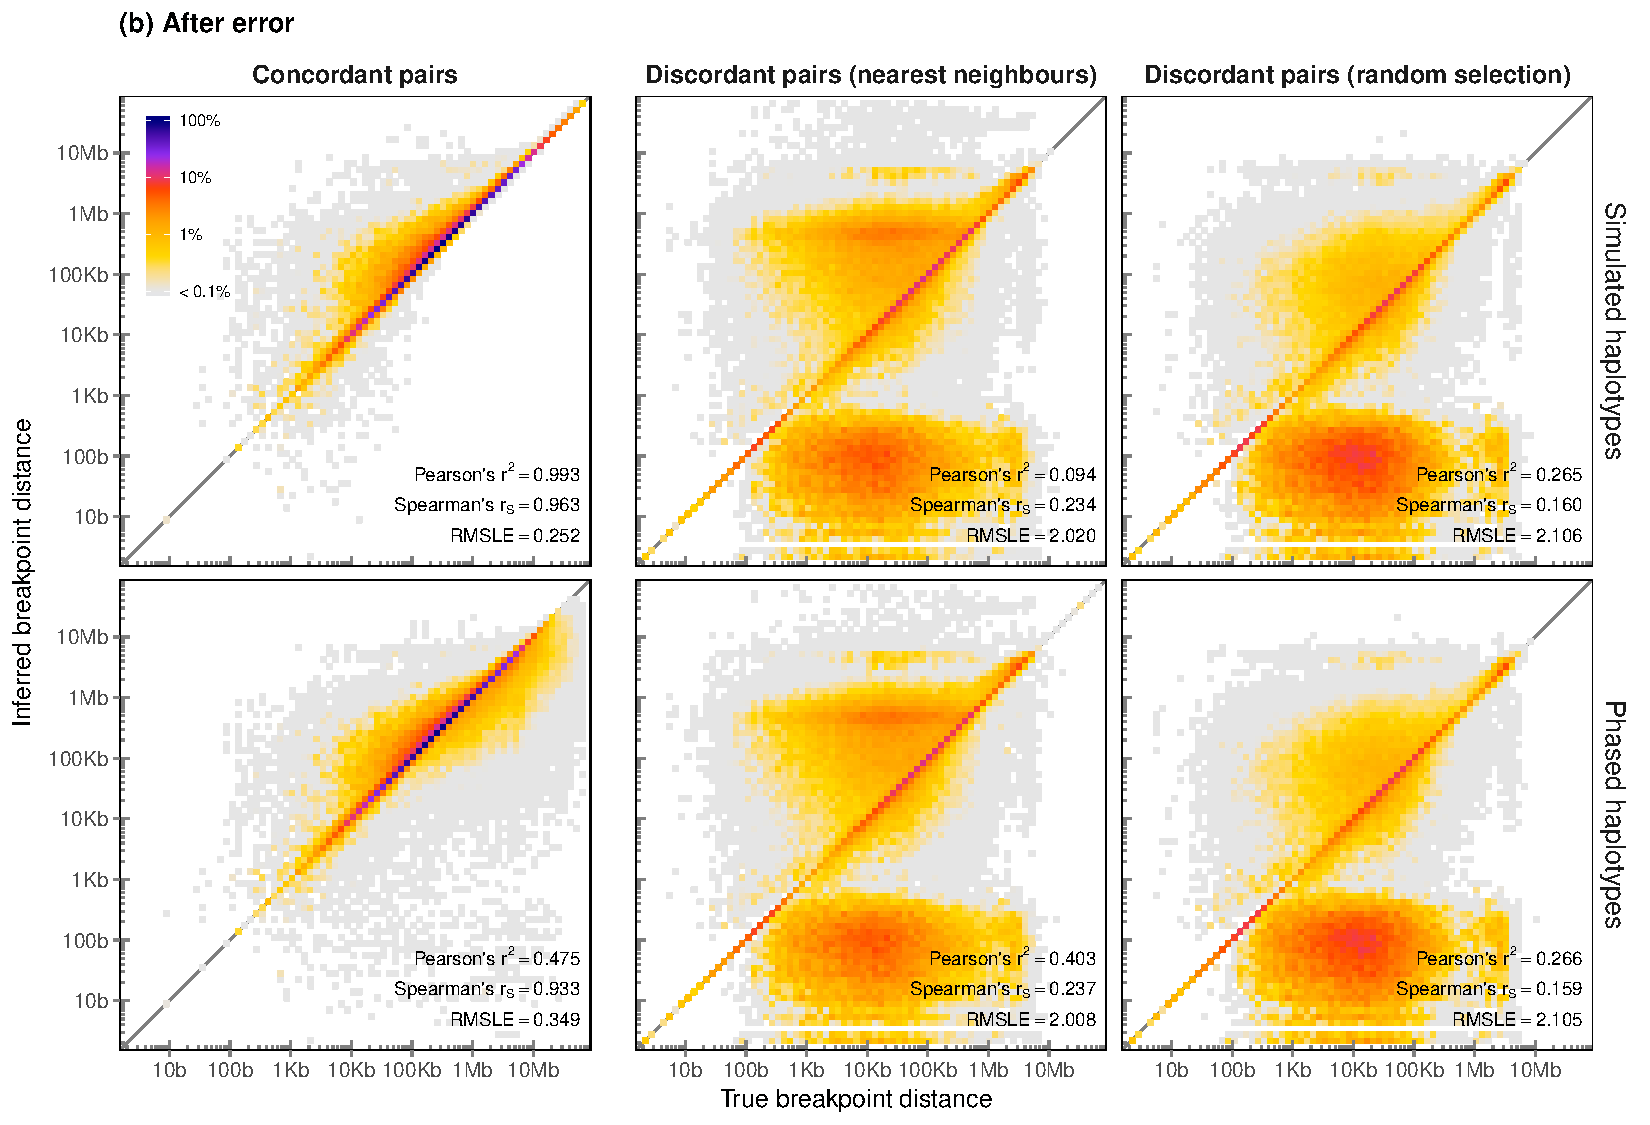
\includegraphics[width=\textwidth]{./img/ch5/hhmm_ibd_rel_B}
\Caption{Density of breakpoint positions inferred using the haplotype-based HMM}
{The physical distance between true and inferred breakpoints (either left or right-hand side) is shown, where colours indicate the maximised density of breakpoints at the relative distance to the focal position, around which a shared haplotype segment was detected.
Pair selection was done using the relaxed nearest neighbour approach and at random.
Note that concordant pairs were selected at random throughout.
Results were obtained on data before \textbf{(a)} and after error \textbf{(b)}, separately on simulated and phased haplotypes.}
{fig:hhmm_ibd_rel}
\end{figure}
